\chapter{OSPF}
\section{Introduction}
\subsection{Link-state operation}
\begin{enumerate}
	\item \textbf{Establish neighbor adjacencies} -- An OSPF-enabled router sends Hello packets out all OSPF-enabled interfaces to determine if neighbors are present on those links. %Process ID and hello/dead timers must match between neighboring OSPF routers in order to form an adjacency.
	\item \textbf{Exchange Link-State Advertisements} -- Routers flood their LSAs (which contain the state and cost of each directly connected link) to adjacent neighbors. Those neighbors then immediately flood the LSAs to other directly connected neighbors, until all routers in the area have all LSAs.
	\item \textbf{Build the Topology Table} -- Routers build the topology table (LSDB) based on the received LSAs.
	\item \textbf{Execute the SPF Algorithm} -- Routers use the SPF algorithm to create the SPF tree.
	\item \textbf{Insert best path to routing table} -- From the SPF tree, the best paths are offered to the IP routing table. The route will be inserted into the routing table unless there is a route source to the same network with a lower administrative distance, such as a static route. Routing decisions are made based on the entries in the routing table, not LSDB.
	\end{enumerate}
\subsection{OSPF network types}
OSPF defines five network types:
\begin{itemize}
	\item \textbf{Point-to-point} -- Two routers interconnected over a common link. No other routers are on the link. (Figure \ref{point-to-point})
	\item \textbf{Multiaccess} -- also called Broadcast multiaccess, Multiple routers interconnected over an Ethernet network. (Figure \ref{multiaccess})
	\item \textbf{Nonbroadcast multiaccess (NBMA)} -- Multiple routers interconnected in a network that does not allow broadcasts, such as Frame Relay. (Figure \ref{NBMA})
	\item \textbf{Point-to-multipoint} -- Multiple routers interconnected in a hub-and-spoke topology over an NBMA network (Figure \ref{point-to-multipoin}).
	\item \textbf{Virtual links} -- Special OSPF network used to interconnect distant OSPF areas to the backbone area (Figure \ref{virtual-link}). In this scenario, area 51 cannot connect directly to area 0. A special OSPF area must be configured to connect area 51 to area 0. The R1 and R2 in area 1 must be configured as a virtual link.
	\end{itemize}
\begin{figure}%
	\centering
	\subfigure[Point-to-point]{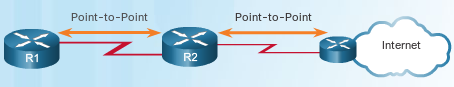
\includegraphics[width=0.4\textwidth]{point-to-point.png} \label{point-to-point}}\qquad%
	\subfigure[Multiaccess]{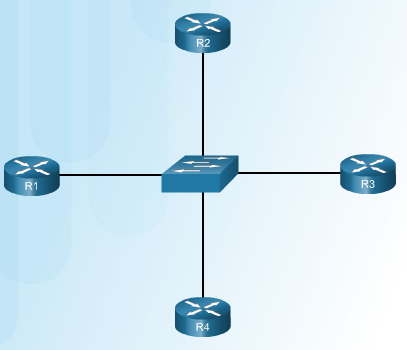
\includegraphics[width=0.4\textwidth]{multiaccess.png} \label{multiaccess}}\\%
	\subfigure[Nonbroadcast multiaccess]{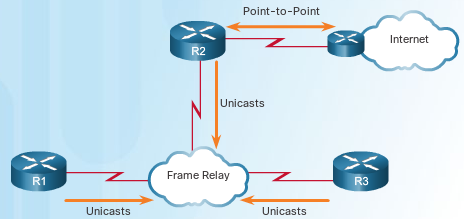
\includegraphics[width=0.4\textwidth]{pictures/NBMA.png} \label{NBMA}}\qquad%
	\subfigure[Point-to-multipoint]{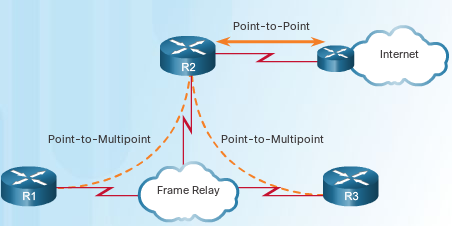
\includegraphics[width=0.4\textwidth]{pictures/point-to-multipoint.png} \label{point-to-multipoin}}
	\subfigure[Virtual link]{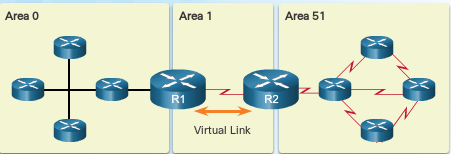
\includegraphics[width=0.4\textwidth]{pictures/virtual-link.png} \label{virtual-link}}
	\caption{OSPF network types}
	\label{network-types}
	\end{figure}
\subsection{OSPF cost}
OSPF uses cost as a metric, where lower cost indicates a better path. The cost of an interface is inversely proportional to the bandwidth of the interface:% Therefore, a higher bandwidth indicates a lower cost. The formula used to calculate the OSPF cost is:
\[ \text{cost}=\frac{\text{Reference bandwidth}}{\text{Interface bandwidth}} \]
The default reference bandwidth is 100 Mb/s, therefore the formula is:
\[ \text{cost}=\frac{10^8}{\text{Interface bandwidth in bps}} \]
Notice that any interfaces faster than 100 Mb/s share the same cost 1, because the OSPF cost value must be an integer. To avoid this, changing reference bandwidth to a higher value than 100 Mb/s is required. \note Changing the reference bandwidth does not actually affect the physical bandwidth of the device; rather, it simply affects the calculation used to determine the metric.

\section{Protocol components}
The OSPF routing protocol has three main components:
\begin{itemize}
	\item Data structures
	\item Routing protocol messages
	\item Algorithm
	\end{itemize}
\subsection{Data structure}
Data structures are the tables or databases that OSPF builds in order to operate. OSPF creates and maintains three databases. These databases are kept and maintained in RAM.
\begin{itemize}
	\item \textbf{Adjacency database} (neighbor table) is a list of all neighbor routers, and unique for each router. It can be viewed using \texttt{show ip ospf neigbor} command.
	\item \textbf{Link-state database or LSDB} (topology table) shows the network topology and is identical for all routers in one area. It can be viewed using \cisco{show ip ospf database} command.
	\item \textbf{Forwarding database} (Routing table) is a list of best routes to reach networks.
\end{itemize}
\subsection{Messages}
OSPF messages are transmitted to multicast address 01-00-5E-00-00-0\textbf{5} and 01-00-5E-00-00-0\textbf{6} in MAC address, 224.0.0.5 and 224.0.0.4 in IPv4, or FF02::5 and FF02::6 in IPv6. The protocol field in IP packet header is set to 89 for OSPF protocol.
OSPF uses five types of packets to convey routing information:
\begin{itemize}
	\item \textbf{Hello packets} establish neighbor adjacency, and facilitate the DR, BDR election in multiaccess network.
	\item \textbf{Database description (DBD) packets} contain an abbreviated LSDB.
	\item \textbf{Link-State Request (LSR) packets} request additional information about network.
	\item \textbf{Link-State Update (LSU) packets} are sent only to neighbors every 30 minutes, or as a response to LSRs, or when a change is perceived.
	\item \textbf{Link-State Acknowledgment (LSAck) packets} are used to confirm receipt of the LSU.
\end{itemize}
\subsubsection{Hello and dead intervals}
The frequency at which the router sends hello packets is specified by hello interval in packet header. The default hello interval on point-to-point and multiaccess network is 10 seconds, on NBMA is 30 seconds. Another important timer is dead interval, which is the period that the router waits to receive a hello packet before declaring the neighbor down. By default, dead interval is four times hello interval. When configuring these two timers on a router, please note that dead interval must be larger than hello interval, and they must be identical on peer routers.
\subsubsection{Link-State Advertisement}
The link-state advertisement (LSA) is a basic communication means of the OSPF routing protocol. It describes a building block of the OSPF LSDB. Individually, they act as database records and provide specific OSPF network details.\par 
LSAs are not Link-State Packets, they are actually packaged inside LSU and DBD packets to convey different kinds of routing information. The use of terms LSU and LSA can sometimes confusing because these terms are often used interchangeably. However, they are different: \emph{An LSU contains one or more LSAs}.\par 
LSA has its own header, which includes link-state type, link's cost, sequence number, the address of advertising router, and link-ID. The \emph{link ID} field identifies the piece of the routing domain based on LSA type (see table \ref{LSA-type}).

\begin{table}[h]
\centering
\caption{Link-State Advertisment types}
\label{LSA-type}
\begin{tabular}{@{} p{2em} p{3em} p{10em} p{5em} p{9em} @{}}
\toprule
LSA type & Sending router & Description                                            & Flooding area        & Link ID                             \\ \midrule
1        & all routers    & Introduce directly connected networks to its neighbors & one area             & router ID of the originating router \\
2        & DR             & Give other routers info about multiaccess network      & one area             & IP interface address of DR		\\
3        & ABR            & Propagates info of each area to all other routers      & between areas        & network address                 \\ 
4        & ABR            & Identify ASBR and provide the route to it              & entire routing domain& router ID of ASBR                 \\ 
5        & ASBR, ABR      & Advertise external network                             & entire routing domain& external network address         \\ \bottomrule
\end{tabular}
\end{table}

\subsection{Algorithm}\label{sec:algorithm}
When an OSPF router is initially connected to a network, it goes through the following states in order:
\begin{enumerate}
	\item \textbf{Down state} (send hello packets but not able to receive them)
	\item \textbf{Init state} (hello packets are received)
	\item \textbf{Two-way state} (elect a DR and a BDR)
	\item \textbf{ExStart state} (decide which router will send the DBD packets first, the router with higher router ID will be the first one to send DBD packets)%negotiate the master/slave relationship and DBD packet sequence number
	\item \textbf{Exchange state} (exchange DBD packets)
	\item \textbf{Loading state} (if the information in DBD packets is different from the LSDB, a router will transition to this state to gain additional route information, using LSRs)
	\item \textbf{Full state} (reach convergence)
\end{enumerate}

\section{DR election}
\begin{description}
	\item[Multiaccess network] Multiaccess networks can create challenges the flooding of LSAs. Ethernet network interconnects routers over a common link, therefore each router considers all counterparts in multiaccess network are its neighbors and establish adjacency to each of them (see figure \ref{multiple-adjacencies}). This could lead to extensive flooding of LSPs when OSPF is initialized or when topology changes occur.
	\item[Designated Router (DR)] The solution to managing the number of adjacencies and the flooding of LSAs on a multiaccess network is the Designated Router (DR). On multiaccess networks, OSPF elects a DR to be the collection and distribution point for LSAs sent and received. The router ID of DR can be viewed using \cisco{show ip ospf interface} command on any routers within the multiaccess network.
	\item[Backup Designated Router (BDR)] A BDR is also elected in case the DR fails. The BDR listens passively to this exchange and maintains a relationship with all the routers. If the DR stops producing Hello packets, the BDR promotes itself and assumes the role of DR.
	\item[DROTHER] All other routers become DROTHER (a router that is neither the DR nor the BDR). DROTHERs only form full adjacencies with the DR and BDR in the network (see figure \ref{DR-adjacency}). Instead of flooding LSAs to all routers in the network, DROTHERs only send their LSAs to the DR and BDR using the multicast address 224.0.0.6 (all DR routers). \\
	To ``keep in touch'' with neighbor routers, DROTHER still form 2-way adjacencies with any DROTHERs that join the multiaccess network. This means that all DROTHER routers in the multiaccess network still receive Hello packets from all other DROTHER routers. In this way, they are aware of all routers in the network.
	\end{description}
\begin{figure}[hbtp]
	\centering
	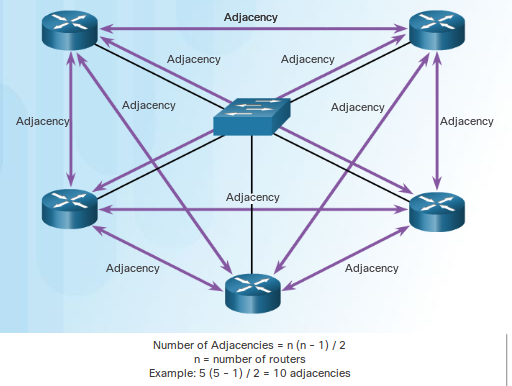
\includegraphics[width=\textwidth]{multiple-adjacencies.png} 
	\caption{Creating adjacencies with every neighbors in multiaccess network}
	\label{multiple-adjacencies}
	\end{figure}
\begin{figure}[hbtp]
	\centering
	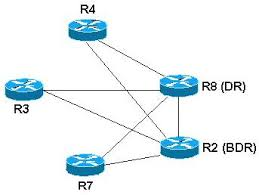
\includegraphics[width=0.4\textwidth]{pictures/dr-bdr.jpeg}
	\caption{DROTHERs only form full adjacencies with the DR and BDR in the network}
	\label{DR-adjacency}
	\end{figure}
The OSPF DR and BDR election decision is based on the following criteria, in sequential order:
\begin{enumerate}
	\item The routers in the network elect the router with the highest interface priority as the DR. The router with the second highest interface priority is elected as the BDR.
	\item If the interface priorities are equal, then the router with the highest router ID is elected the DR. The router with the second highest router ID is the BDR.
	\end{enumerate}
OSPF DR and BDR elections are not pre-emptive. If a new router with a higher priority or higher router ID is added to the network after the DR and BDR election, the newly added router does not take over the DR or the BDR role. This is because those roles have already been assigned. The addition of a new router does not initiate a new election process.\par 
If the DR fails, the BDR is automatically promoted to DR. This is the case even if another DROTHER with a higher priority or router ID is added to the network after the initial DR/BDR election. However, after a BDR is promoted to DR, a new BDR election occurs and the DROTHER with the higher priority or router ID is elected as the new BDR.
After the DR is elected, it remains the DR until one of the following events occurs:
\begin{itemize}
	\item The DR fails
	\item The OSPF process on the DR fails or is stopped
	\item The multiaccess interface on the DR fails or is shutdown
	\end{itemize}


\section{Multiarea OSPF}
\subsection{Single-area vs Multi-area OSPF}
An OSPF area is a group of routers that share the same link-state information in their LSDBs.
Single-area OSPF is useful in smaller networks, however, if an area becomes too big, the following issues must be addressed:
\begin{itemize}
	\item Large routing table (no summarization by default)
	\item Large link-state database (contains the entire network topology)
	\item Frequent SPF algorithm calculations (even small changes in a specific area of the network makes the routers recalculate the SPF algorithm and update the LSDB for the entire routing domain.)
	\end{itemize}
Multiarea OSPF have these advantages:
\begin{itemize}
	\item Smaller routing table (There are fewer routing table entries as network addresses can be summarized between areas.)
	\item Reduced link-state update overhead (Fewer routers exchanging LSAs because LSA flooding stops at the area boundary.)
	\item Reduced frequency of SPF calculations (Routing still occurs between the areas, however, the CPU intensive routing operation of recalculating the SPF algorithm is done only for routes within an area.)
	\end{itemize}
	
\subsection{Introduction to multiarea OSPF}
\subsubsection{Two-layer area hierarchy}
To make OSPF more efficient and scalable, Multiarea OSPF is implemented in a two-layer area hierarchy:
\begin{itemize}
	\item \textbf{Backbone (Transit) area} -- A backbone area directly connected with all other areas. All traffic moving from one area to another area must traverse the backbone area. Generally, end users are not found within a backbone area. The backbone area is also called OSPF area 0.
	\item \textbf{Regular (Non-backbone) area} -- Connects users and resources. By default, a regular area does not allow traffic from another area to use its links to reach other areas. All traffic from other areas must cross a transit area.
	\end{itemize}
	
\subsubsection{Types of routers}
There are four different types of OSPF routers:
\begin{itemize}
	\item Internal router (have all interfaces in the same area)
	\item Backbone router (reside in backbone area)
	\item Area border router or ABR (have interfaces attached to multiple areas)
	\item Autonomous System Boundary Router or ASBR (have at least one interface attached to an external network)
	\end{itemize}

\subsubsection{Multiarea configuration}
The optimal number of routers per area varies based on factors such as network stability, but Cisco recommends the following guidelines:
\begin{itemize}
	\item An area should have no more than 50 routers.
	\item A router should not be in more than three areas.
	\item Any single router should not have more than 60 neighbors.
	\end{itemize}

Also keep the following notes in mind:
\begin{itemize}
	\item Propagating type 3 and 5 LSAs can cause significant flooding problems. For this reason, it is strongly recommended that manual route summarization be configured on the ABRs and ASBR.
	\item Receiving a type 3 LSA does not cause a router to run the SPF algorithm, but the routes being advertised in the type 3 LSAs are appropriately updated to the routing table.
	\item In the routing table, OSPF intra-area routes start with O, inter-area routes start with O IA, external routes start with O E1 (or O E2).
	\item SPF algorithm calculates the best paths in order: calculate intra-area routes $\rightarrow$ calculate inter-area routes $\rightarrow$ calculate external routes.
	\end{itemize}

